\documentclass{beamer}
\usetheme{Warsaw}
\usecolortheme{seahorse}
\usepackage{amsmath}
\usepackage{amsfonts}
\usepackage{epstopdf}
\usepackage{amssymb}
\usepackage{graphicx}
\usepackage{movie15}
%\usepackage{CJKutf8}
\title{Introduction to Fourier transform and signal analysis}
\author{\texorpdfstring{Zong-han, Xie\newline\url{icbm0926@gmail.com}}{Zong-han, Xie}}
\begin{document}
%\begin{CJK}{UTF8}{cwmc}
\begin{frame}
\titlepage
\end{frame}
\begin{frame}[label=licensepage]
\frametitle{License of this document}
Introduction to Fourier transform and signal analysis by Zong-han, Xie (\href{icbm0926@gmail.com}{icbm0926@gmail.com}) is licensed under a Creative Commons Attribution-NonCommercial 4.0 International License. \newline
\begin{center}
\includegraphics[scale=1]{by-nc-sa.eps}
\end{center}
\end{frame}
\AtBeginSection[]
{
  \begin{frame}
    \frametitle{Outline}
    \tableofcontents[currentsection]
  \end{frame}
}
\section{Continuous Fourier transform}
\begin{frame}
\frametitle{Orthogonal condition}
\begin{itemize}
\item Any two vectors $\mathbf{a}$, $\mathbf{b}$ satisfied the following condition are mutually orthogonal. \newline
\begin{eqnarray}
\mathbf{a}^* \cdot \mathbf{b} = 0
\label{eq:ortho_vec}
\end{eqnarray}
\item Any two functions $a(x)$, $b(x)$ satisfied the following condition are mutually orthogonal. \newline
\begin{eqnarray}
\int{a^*(x)} \cdot {b(x)} dx = 0
\label{eq:ortho_func}
\end{eqnarray}
\item * means complex conjugate. \newline
\end{itemize}
\end{frame}
\begin{frame}
\frametitle{Complete and orthogonal basis}
\begin{itemize}
\item $\cos nx $ and $\sin mx$ are mutually orthogonal in which n and m are integers.
\begin{eqnarray}
\int_{-\pi}^{\pi}{\cos nx} \cdot {\sin mx} dx = 0 \nonumber \\
\int_{-\pi}^{\pi}{\cos nx} \cdot {\cos mx} dx = \pi\delta_{nm} \nonumber \\
\int_{-\pi}^{\pi}{\sin nx} \cdot {\sin mx} dx = \pi\delta_{nm}
\end{eqnarray}
\item $\delta_{nm} $ is Dirac-delta symbol. It means $\delta_{nn} = 1$ and $\delta_{nm} = 0$ when $n \neq m$.
\end{itemize}
\end{frame}
\begin{frame}
\frametitle{Fourier series}
Since $\cos nx $ and $\sin mx$ are mutually orthogonal, we can expand an arbitrary periodic function $f(x)$ by them. we shall have a series expansion of $f(x)$ which has $2\pi$ period.
\begin{eqnarray}
f(x)&=&a_0 + \sum_{k=1}^{\infty} \left(a_k\cos kx + b_k \sin kx\right) \nonumber \\
a_0&=&\frac{1}{2\pi}\int_{-\pi}^{\pi}f(x) dx \nonumber \\
a_k&=&\frac{1}{\pi}\int_{-\pi}^{\pi}f(x) \cos kx dx \nonumber \\
b_k&=&\frac{1}{\pi}\int_{-\pi}^{\pi}f(x) \sin kx dx
\label{eq:fseries}
\end{eqnarray}
\end{frame}
\begin{frame}
\frametitle{Fourier series}
If $f(x)$ has $L$ period instead of $2\pi$, $x$ is replaced with $\pi x /L$.
\begin{eqnarray}
f(x)&=&a_0 + \sum_{k=1}^{\infty} \left(a_k\cos \frac{2k\pi x}{L} + b_k \sin \frac{2k\pi x}{L}\right) \nonumber \\
a_0&=&\frac{1}{L}\int_{-\frac{L}{2}}^{\frac{L}{2}}f(x) dx \nonumber \\
a_k&=&\frac{2}{L}\int_{-\frac{L}{2}}^{\frac{L}{2}}f(x) \cos \frac{2k\pi x}{L} dx, k = 1,2,...\nonumber \\
b_k&=&\frac{2}{L}\int_{-\frac{L}{2}}^{\frac{L}{2}}f(x) \sin \frac{2k\pi x}{L} dx, k = 1,2,...
\label{eq:fseries_pL}
\end{eqnarray}
\end{frame}
\begin{frame}
\frametitle{Complex Fourier series}
Using Euler's formula, equation (\ref{eq:fseries}) becomes 
\begin{eqnarray}
f(x)=a_0 + \sum_{k=1}^{\infty} \left(\frac{a_k - ib_k}{2} e^{ikx} + \frac{a_k + ib_k}{2}e^{-ikx}\right) \nonumber
\end{eqnarray}
Let $c_0 \equiv a_0$, $c_k \equiv \frac{a_k - ib_k}{2}$ and $c_{-k} \equiv \frac{a_k + ib_k}{2}$, we have
\begin{eqnarray}
f(x)&=&\sum_{m=-\infty}^{\infty} c_m e^{imx} \nonumber \\
c_m&=&\frac{1}{2\pi}\int_{-\pi}^{\pi} f(x) e^{-imx} dx
\label{eq:cfseries}
\end{eqnarray}
$e^{imx}$ and $e^{inx}$ are also mutually orthogonal provided $n \neq m$ and it forms a complete set. Therfore, it can be used as orthogonal basis.\newline
\end{frame}
\begin{frame}
\frametitle{Complex Fourier series}
If $f(x)$ has $T$ period instead of $2\pi$, $x$ is replaced with $2\pi x /T$.
\begin{eqnarray}
f(x)&=&\sum_{m=-\infty}^{\infty} c_m e^{i\frac{2\pi mx}{T}} \nonumber \\
c_m&=&\frac{1}{T}\int_{-\frac{T}{2}}^{\frac{T}{2}} f(x) e^{-i\frac{2\pi mx}{T}} dx, m = 0,1,2...
\label{eq:cfseries_pT}
\end{eqnarray}
\end{frame}
\begin{frame}
\frametitle{Fourier Series of step function}
$f(x)$ is a periodic function with $2\pi$ period and it's defined as follows.
\begin{eqnarray}
f(x)&=& 0, -\pi < x < 0 \nonumber \\
f(x)&=& h, 0 < x < \pi
\label{eq:stepfunc}
\end{eqnarray}
Fourier series of $f(x)$ is
\begin{eqnarray}
f(x)= \frac{h}{2} + \frac{2h}{\pi} \left( \frac{\sin x}{1} + \frac{\sin 3x}{3} + \frac{\sin 5x}{5} + ...\right)
\label{eq:stepfunc_ft}
\end{eqnarray}
$f(x)$ is piecewise continuous within the periodic region. Fourier series of $f(x)$ converges at speed of $1/n$.
\end{frame}
\begin{frame}
\frametitle{Fourier series of step function}
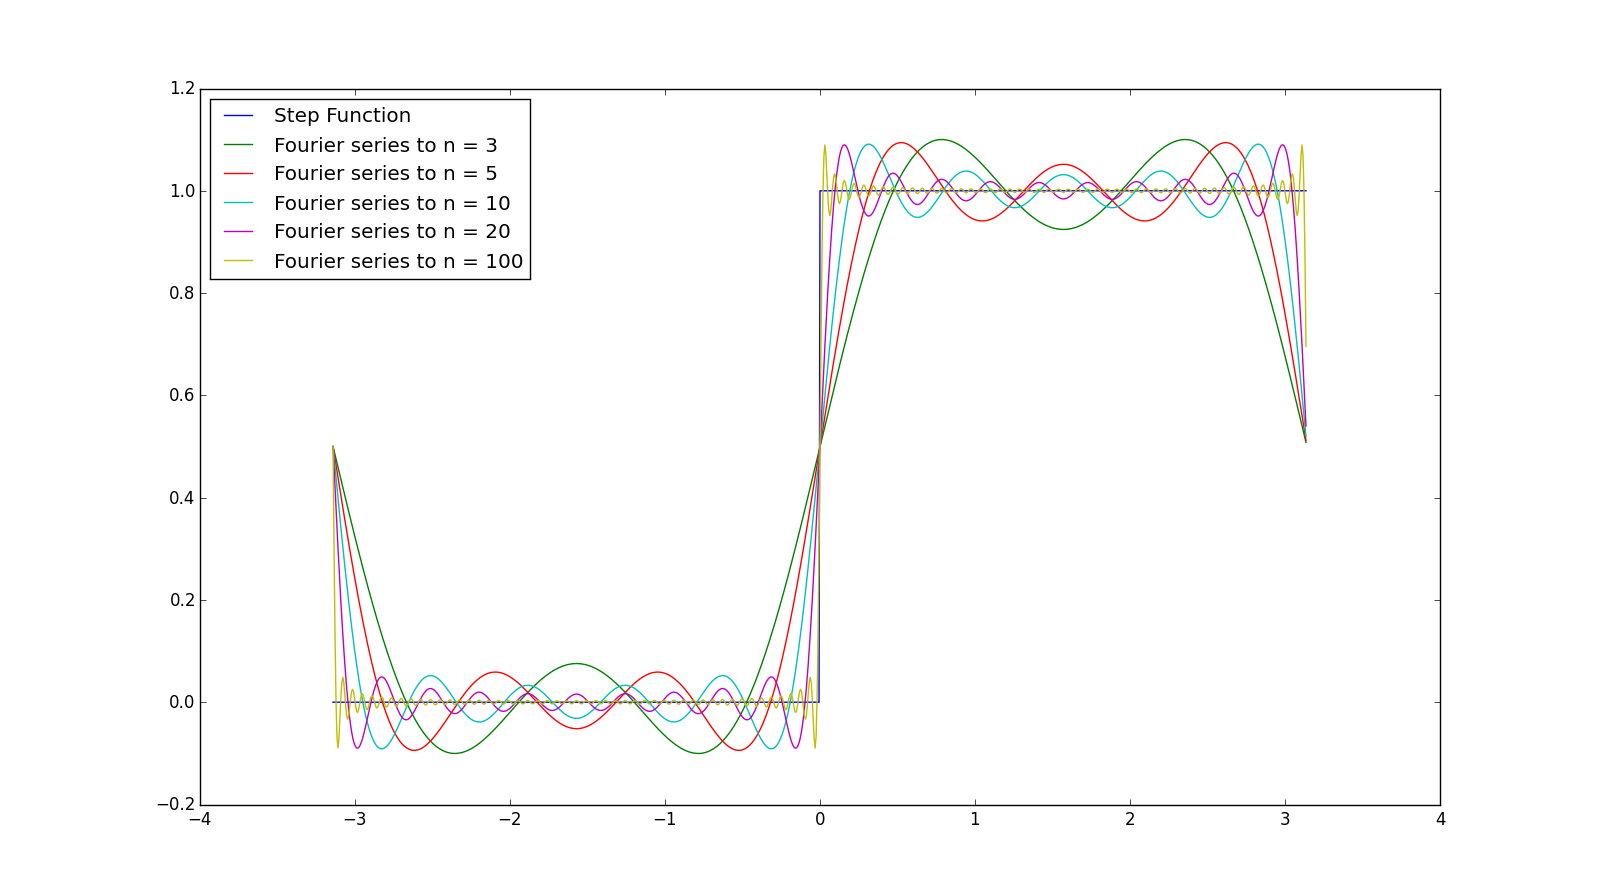
\includegraphics[scale=0.3]{step.png}
\end{frame}
\begin{frame}
\frametitle{Fourier series of saw tooth function}
$f(x)$ is a periodic function with $2\pi$ period and it's defined as follows.
\begin{eqnarray}
f(x)&=& -x, -\pi < x < 0 \nonumber \\
f(x)&=& x, 0 < x < \pi
\label{eq:sawfunc}
\end{eqnarray}
Fourier series of $f(x)$ is
\begin{eqnarray}
f(x)= \frac{\pi}{2} - \frac{4}{\pi} \sum_{n=1,3,5...} \left( \frac{\cos nx}{n^2} \right)
\label{eq:sawfunc_ft}
\end{eqnarray}
$f(x)$ is continuous and its derivative is piecewise continuous within the periodic region. Fourier series of $f(x)$ converges at speed of $1/n^2$.
\end{frame}
\begin{frame}
\frametitle{Fourier series of saw tooth function}
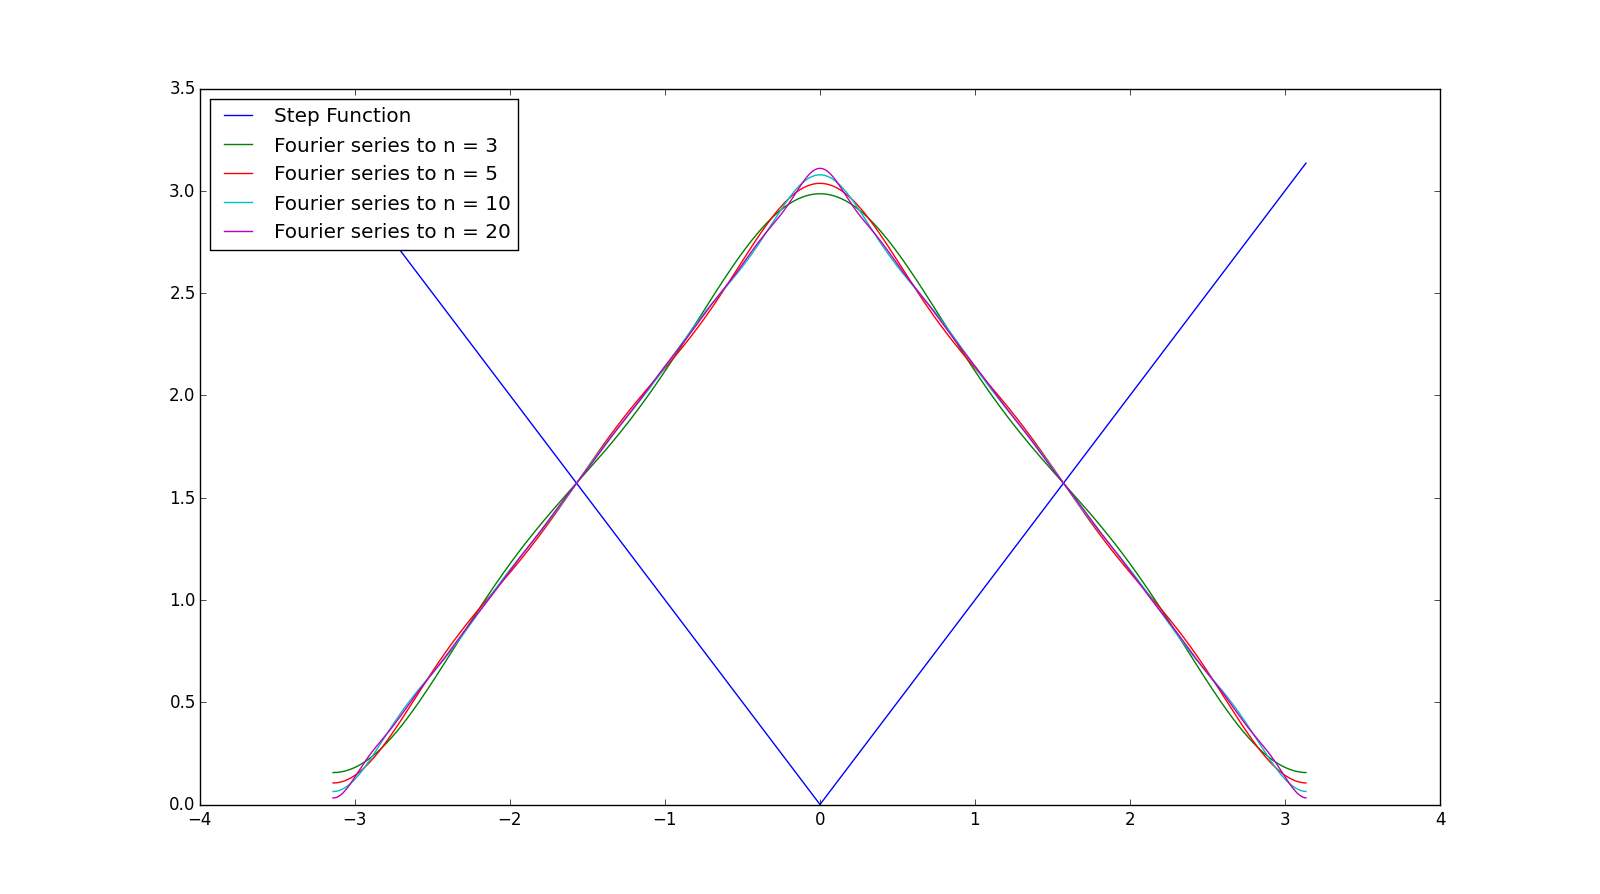
\includegraphics[scale=0.3]{sawtooth.png}
\end{frame}
\begin{frame}
\frametitle{Fourier series of full wave rectifier}
$f(t)$ is a periodic function with $2\pi$ period and it's defined as follows.
\begin{eqnarray}
f(t)&=& -\sin {\omega t}, -\pi < t < 0 \nonumber \\
f(t)&=& \sin {\omega t}, 0 < t < \pi
\label{eq:fullrectifier_func}
\end{eqnarray}
Fourier series of $f(x)$ is
\begin{eqnarray}
f(t)= \frac{2}{\pi} - \frac{4}{\pi} \sum_{n=2,4,6...} \left( \frac{\cos n\omega t}{n^2 - 1} \right)
\label{eq:fullrectifier_func_ft}
\end{eqnarray}
$f(x)$ is continuous and its derivative is piecewise continuous within the periodic region. Fourier series of $f(x)$ converges at speed of $1/n^2$.
\end{frame}
\begin{frame}
\frametitle{Fourier series of full wave rectifier}
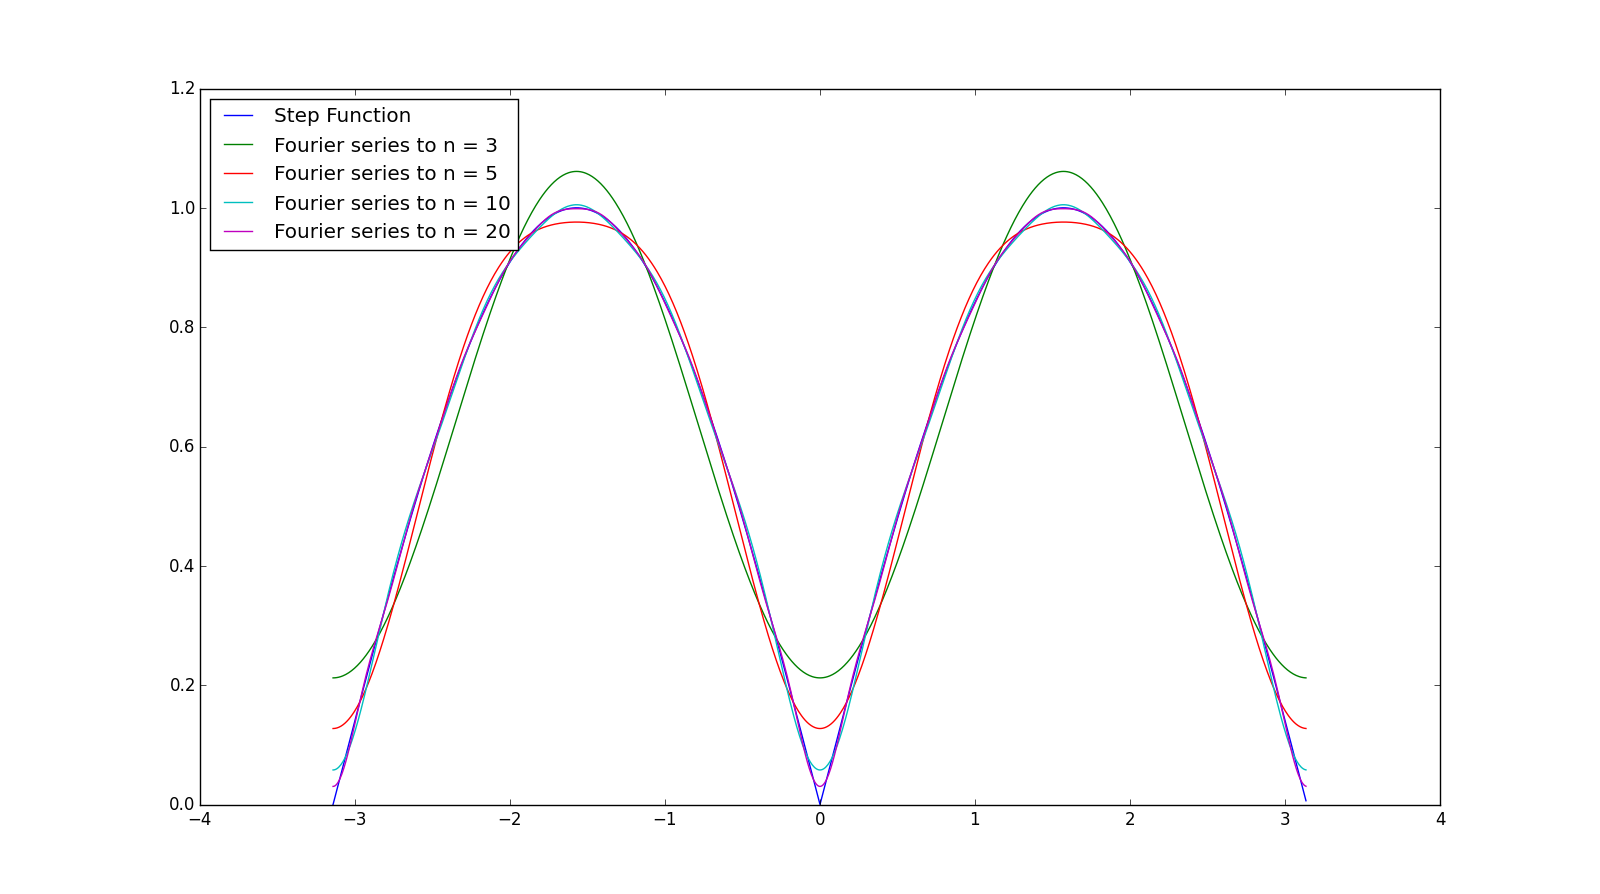
\includegraphics[scale=0.3]{fullrectifier.png}
\end{frame}
\begin{frame}
\frametitle{Fourier transform}
from Eq. \ref{eq:cfseries_pT}, we define variables $k \equiv \frac{2\pi m}{T}$, $\hat{f}(k) \equiv\frac{c_mT}{\sqrt{2\pi}}$ and $ \bigtriangleup{k} \equiv \frac{2\pi (m+1)}{T} - \frac{2\pi m}{T} = \frac{2\pi}{T}$. \newline We can have
\begin{eqnarray}
f(x)&=&\frac{1}{\sqrt{2\pi}}\sum_{m=-\infty}^{\infty} \hat{f}(k) e^{ikx} \bigtriangleup{k} \nonumber \\
\hat{f}(k)&=&\frac{1}{\sqrt{2\pi}}\int_{-\frac{T}{2}}^{\frac{T}{2}} f(x) e^{-ikx}dx\nonumber
\end{eqnarray}
\end{frame}
\begin{frame}
\frametitle{Fourier transform}
Let $T\longrightarrow\infty$
\begin{eqnarray}
f(x)&=&\frac{1}{\sqrt{2\pi}}\int_{-\infty}^{\infty} \hat{f}(k) e^{ikx} dk
\label{eq:ftransform_inv}\\
\hat{f}(k)&=&\frac{1}{\sqrt{2\pi}}\int_{-\infty}^{\infty} f(x) e^{-ikx} dx
\label{eq:ftransform}
\end{eqnarray}
Eq.\ref{eq:ftransform} is the \emph{Fourier transform} of $f(x)$ and Eq.\ref{eq:ftransform_inv} is the \emph{inverse Fourier transform} of $\hat{f}(k)$.
\end{frame}
\begin{frame}
\frametitle{Properties of Fourier transform}
$f(x)$, $g(x)$ and $h(x)$ are functions and  their Fourier transforms are $\hat{f}(k)$, $\hat{g}(k)$ and $\hat{h}(k)$. $a$, $b$ $x_0$ and $k_0$ are real numbers.
\begin{itemize}
\item Linearity: If $h(x) = af(x)+bg(x)$, then Fourier transform of $h(x)$ equals to $\hat{h}(k) = a\hat{f}(k)+b\hat{g}(k)$.
\item Translation: If $h(x) = f(x-x_0)$, then $\hat{h}(k) = \hat{f}(k)e^{-ikx_0}$
\item Modulation: If $h(x) = e^{ik_0x}f(x)$, then $\hat{h}(k) = \hat{f}(k-k_0)$
\item Scaling: If $h(x) = f(ax)$, then $\hat{h}(k) = \frac{1}{a}\hat{f}(\frac{k}{a})$
\item Conjugation: If $h(x) = f^*(x)$, then $\hat{h}(k) = \hat{f}^*(-k)$. With this property, one can know that if $f(x)$ is real and then $\hat{f}^*(-k) = \hat{f}(k)$. One can also find that if $f(x)$ is real and then $|\hat{f}(k)| = |\hat{f}(-k)|$.
\end{itemize}
\end{frame}
\begin{frame}
\frametitle{Properties of Fourier transform}
\begin{itemize}
\item If $f(x)$ is even, then $\hat{f}(-k) = \hat{f}(k)$.
\item If $f(x)$ is odd, then $\hat{f}(-k) = -\hat{f}(k)$.
\item If $f(x)$ is real and even, then $\hat{f}(k)$ is real and even.
\item If $f(x)$ is real and odd, then $\hat{f}(k)$ is imaginary and odd.
\item If $f(x)$ is imaginary and even, then $\hat{f}(k)$ is imaginary and even.
\item If $f(x)$ is imaginary and odd, then $\hat{f}(k)$ is real and odd.
\end{itemize}
\end{frame}
\begin{frame}
\frametitle{Dirac delta function}
Dirac delta function is a generalized function defined as the following equation.
\begin{eqnarray}
f(0) &=&\int_{-\infty}^{\infty} f(x)\delta{(x)} dx \nonumber \\
\int_{-\infty}^{\infty}\delta{(x)} dx &=& 1
\label{eq:dirac_delta}
\end{eqnarray}
The Dirac delta function can be loosely thought as a function which equals to infinite at $x = 0$ and to zero else where.
\begin{eqnarray}
\delta(x) = \begin{cases} +\infty, & x = 0 \\ 0, & x \ne 0 \end{cases} \nonumber
\end{eqnarray}
\end{frame}
\begin{frame}
\frametitle{Dirac delta function}
From Eq.\ref{eq:ftransform} and Eq.\ref{eq:ftransform_inv}
\begin{eqnarray}
\hat{f}(k)&=&\frac{1}{2\pi}\int_{-\infty}^{\infty} \int_{-\infty}^{\infty} \hat{f}(k') e^{ik'x} dk' e^{-ikx} dx \nonumber \\
          &=&\frac{1}{2\pi}\int_{-\infty}^{\infty} \int_{-\infty}^{\infty} \hat{f}(k') e^{i(k'-k)x} dx dk' \nonumber
\end{eqnarray}
Comparing to "Dirac delta function", we have
\begin{eqnarray}
\hat{f}(k)&=&\int_{-\infty}^{\infty} \hat{f}(k') \delta{(k'- k)} dk' \nonumber \\
\delta{(k'- k)} &=& \frac{1}{2\pi}\int_{-\infty}^{\infty} e^{i(k'-k)x} dx
\label{eq:dirac_delta_fourier}
\end{eqnarray}
Eq.\ref{eq:dirac_delta_fourier} doesn't converge by itself, it is only well defined as part of an integrand.
\end{frame}
\begin{frame}
\frametitle{Convolution theory}
Considering two functions $f(x)$ and $g(x)$ with their Fourier transform $F(k)$ and $G(k)$. We define an operation
\begin{eqnarray}
f\ast g = \int_{-\infty}^{\infty}g(y)f(x-y)dy
\label{eq:convolution}
\end{eqnarray}
as the convolution of the two functions $f(x)$ and $g(x)$ over the interval $\{ -\infty \sim \infty \}$. It satisfies the following relation:
\begin{eqnarray}
f \ast g = \int_{-\infty}^{\infty}F(k)G(k) e^{ikx}dt
\label{eq:convolution_theorem}
\end{eqnarray}
Let $h(x)$ be $f \ast g$ and $\hat{h}(k)$ be the Fourier transform of $h(x)$, we have
\begin{eqnarray}
\hat{h}(k) = \sqrt{2\pi}F(k)G(k)
\label{eq:convolution_theorem2}
\end{eqnarray}
\end{frame}
\begin{frame}
\frametitle{Parseval relation}
\begin{eqnarray}
\int_{-\infty}^{\infty}f(x)g(x)^* dx &=&\int_{-\infty}^{\infty}  \frac{1}{\sqrt{2\pi}} \int_{-\infty}^{\infty} F(k) e^{ikx}dk \frac{1}{\sqrt{2\pi}} \nonumber \\
&&\int_{-\infty}^{\infty}G^*(k') e^{-ik'x}dk' dx\nonumber \\
&=&\int_{-\infty}^{\infty} \frac{1}{2\pi} \int_{-\infty}^{\infty} F(k)G^*(k')e^{i(k-k')x} dk dk' \nonumber
\end{eqnarray}
By using \ref{eq:dirac_delta_fourier}, we have the Parseval's relation.
\begin{eqnarray}
\int_{-\infty}^{\infty}f(x)g^*(x) dx &=& \int_{-\infty}^{\infty}F(k)G^*(k)dk
\label{eq:parseval_relation}
\end{eqnarray}
Calculating inner product of two fuctions gets same result as the inner product of their Fourier transform.
\end{frame}
\begin{frame}
\frametitle{Cross-correlation}
Considering two functions $f(x)$ and $g(x)$ with their Fourier transform $F(k)$ and $G(k)$. We define cross-correlation as
\begin{eqnarray}
(f\star g)(x) = \int_{-\infty}^{\infty}f^*(x+y)g(x)dy
\label{eq:cross_correlation}
\end{eqnarray}
as the cross-correlation of the two functions $f(x)$ and $g(x)$ over the interval $\{ -\infty \sim \infty \}$. It satisfies the following relation:
Let $h(x)$ be $f \star g$ and $\hat{h}(k)$ be the Fourier transform of $h(x)$, we have
\begin{eqnarray}
\hat{h}(k) = \sqrt{2\pi}F^*(k)G(k)
\label{eq:cross_correlation_FT}
\end{eqnarray}
Autocorrelation is the cross-correlation of the signal with itself.
\begin{eqnarray}
(f\star f)(x) = \int_{-\infty}^{\infty}f^*(x+y)f(x)dy
\label{eq:autocorrelation}
\end{eqnarray}
\end{frame}
\begin{frame}
\frametitle{Uncertainty principle}
One important properties of Fourier transform is uncertainty principle. It states that the more concentrated $f(x)$ is, the more spread its Fourier transform $\hat{f}(k)$ is.
Without loss of generality, we consider $f(x)$ as a normalized function which means $\int_{-\infty}^{\infty}|f(x)|^2 dx = 1$, we have uncertainty relation:
\begin{eqnarray}
\left( \int_{-\infty}^{\infty}(x-x_0)^2|f(x)|^2 dx\right) \left( \int_{-\infty}^{\infty}(k-k_0)^2|\hat{f}(k)|^2 dk\right) \geqq \frac{1}{16\pi^2}
\label{eq:uncertainty_wiki}
\end{eqnarray}
for any $x_0$ and $k_0$ $\in \mathbf{R}$.~\cite{wiki_FT}
\end{frame}
\begin{frame}
\frametitle{Fourier transform of a Gaussian function}

\end{frame}
\begin{frame}
\frametitle{Fourier transform of a Gaussian function with carrier}
\end{frame}
\begin{frame}
\frametitle{Transfer function}

\end{frame}
\section{Discrete Fourier transform}
\begin{frame}
\frametitle{Nyquist critical frequency}
Critical sampling of a sine wave is two sample points per cycle. This leads to \emph{Nyquist critical frequency} $f_c$.
\begin{eqnarray}
f_c &=& \frac{1}{2\Delta}
\label{eq:Nyquist_frequency}
\end{eqnarray}
Where $\Delta$ is the sampling interval. Sampling theorem: If a continuos signal $h(t)$ sampled with interval $\Delta$ happens to be bandwidth limited to frequencies smaller than $f_c$. $h(t)$ is completely determined by its samples $h_n$
\begin{eqnarray}
h(t) &=& \Delta \sum_{n=-\infty}^{\infty} h_n \frac{\sin [2\pi f_c(t-n\Delta)]}{\pi (t-n\Delta)}
\label{eq:sampling_theorem}
\end{eqnarray}
\end{frame}
\begin{frame}
\frametitle{Discrete Fourier transform}
Signal $h(t)$ is sampled with N consecutive values and sampling interval $\Delta$. We have $h_k \equiv h(t_k)$ and $t_k \equiv k*\Delta$, $k = 0,1,2,...,N-1$. \\
With N discrete input, we evidently can only output independent values no more than N. Therefore, we seek for frequencies with values
\begin{eqnarray}
f_n \equiv \frac{n}{N\Delta}, n = -\frac{N}{2}, ...,\frac{N}{2}
\label{eq:DFT_Frequencies}
\end{eqnarray}
\end{frame}
\begin{frame}
\frametitle{Discrete Fourier transform}
Fourier transform of Signal $h(t)$ is $H(f)$. We have discrete Fourier transform $H_n$.
\begin{eqnarray}
H(f_n)&=&\int_{-\infty}^{\infty}h(t)e^{-i2\pi f_nt}dt \approx \Delta \sum_{k=0}^{N-1}h_ke^{-i2\pi f_nt_k} \nonumber \\
&=& \Delta \sum_{k=0}^{N-1}h_ke^{-i2\pi kn/N} \nonumber \\
H_n &\equiv& \sum_{k=0}^{N-1}h_ke^{-i2\pi kn/N}
\label{eq:dft}
\end{eqnarray}
Inverse Fourier transform is
\begin{eqnarray}
h_k &\equiv& \frac{1}{N}\sum_{n=0}^{N-1}H_ne^{i2\pi kn/N}
\label{eq:idft}
\end{eqnarray}
%Discrete form of Parseval's relation is 
%\begin{eqnarray}
%\sum_{k=0}^{N-1}|h_k|^2 = \frac{1}{N}\sum_{n=0}^{N-1}|H_n|^2
%\label{eq:discrete_parseval}
\end{eqnarray}
\end{frame}
\begin{frame}
\frametitle{Periodicity of discrete Fourier transform}
From Eq.\ref{eq:dft}, if we substitute $n$ with $n+N$, we have $H_n = H_{n+N}$. Therefore, discrete Fourier transform has periodicity of $N$.
\begin{eqnarray}
H_{n+N} &=& \sum_{k=0}^{N-1}h_ke^{-i2\pi k(n+N)/N} \nonumber \\
&=&\sum_{k=0}^{N-1}h_ke^{-i2\pi k(n)/N}e^{-i2\pi kN/N} \nonumber \\
&=&H_n
\end{eqnarray}
Critical frequency $f_c$ corresponds to $\frac{1}{2\Delta}$.
\end{frame}
\begin{frame}
\frametitle{Aliasing}

\end{frame}
\begin{frame}
\frametitle{Fast Fourier transform}
\end{frame}
\section{Calculate DFT with Python Numpy Package}
\begin{frame}
\frametitle{Discrete Fourier transform in Numpy or Scipy}

\end{frame}
\begin{frame}
\frametitle{Transform one dimensional data}
\end{frame}
\begin{frame}
\frametitle{Transform more than one dimensional data}
\end{frame}
\section{References}
\begin{frame}
\frametitle{References}
\begin{thebibliography}{7}
\bibitem{SNGP} Supplementary Notes of General Physics by Jyhpyng Wang, \url{http://idv.sinica.edu.tw/jwang/SNGP/SNGP20090621.pdf}
\bibitem{wiki_FS} \url{http://en.wikipedia.org/wiki/Fourier_series}
\bibitem{wiki_FT} \url{http://en.wikipedia.org/wiki/Fourier_transform}
\bibitem{arfken} MATHEMATICAL METHODS FOR PHYSICISTS by George B. Arfken and Hans J. Weber. ISBN-13: 978-0120598762
\bibitem{nr_3rd} Numerical Recipes 3rd Edition: The Art of Scientific Computing by William H. Press  (Author), Saul A. Teukolsky. ISBN-13: 978-0521880688
\bibitem{nr_3rd_web} Chapter 12 and 13 in \url{http://www.nrbook.com/a/bookcpdf.php}
\bibitem{scipy_fft}http://docs.scipy.org/doc/scipy-0.14.0/reference/fftpack.html
\bibitem{scipy_signal}http://docs.scipy.org/doc/scipy-0.14.0/reference/signal.html
\end{thebibliography}
\end{frame}
\begin{frame}
\frametitle{References}
\begin{thebibliography}{1}
\bibitem{DSP_book} Digital Signal Processing: A Computer-Based Approach, 3e by Sanjit K. Mitra
\end{thebibliography}
\end{frame}
\section{}
%---------------Examples of Latex---------
%\begin{frame}
%\frametitle{2nd page}
%\begin{block}{block}
%\begin{eqnarray}
%\frac{1}{2}
%\end{eqnarray}
%\end{block}
%\begin{alertblock}{alertblock}
%alertblock content
%\end{alertblock}
%\end{frame}
%\begin{frame}
%\frametitle{3rd page}
%\begin{itemize}
%\item<1-> 第一
%\item<1-> 2nd
%\item<2-> 3rd
%\item<3-> etc.
%\hyperlink{1stpage}{\beamerbutton{go fuck}}
%\end{itemize}
%\end{frame}
%\end{CJK}
\end{document}
